\documentclass{standalone}

\usepackage{mathtools}
\usepackage{amsmath}
\usepackage{amssymb}
\usepackage{amsfonts}

\usepackage{tikz}
\usepackage{scalerel}
\usepackage{pict2e}
\usepackage{tkz-euclide}
\usetikzlibrary{calc}
\usetikzlibrary{patterns, arrows.meta}
\usetikzlibrary{shadows}
\usetikzlibrary{external}

\usepackage{pgfplots}
\pgfplotsset{compat=newest}
\usepgfplotslibrary{statistics}
\usepgfplotslibrary{fillbetween}

\usepackage{xcolor}


\begin{document}

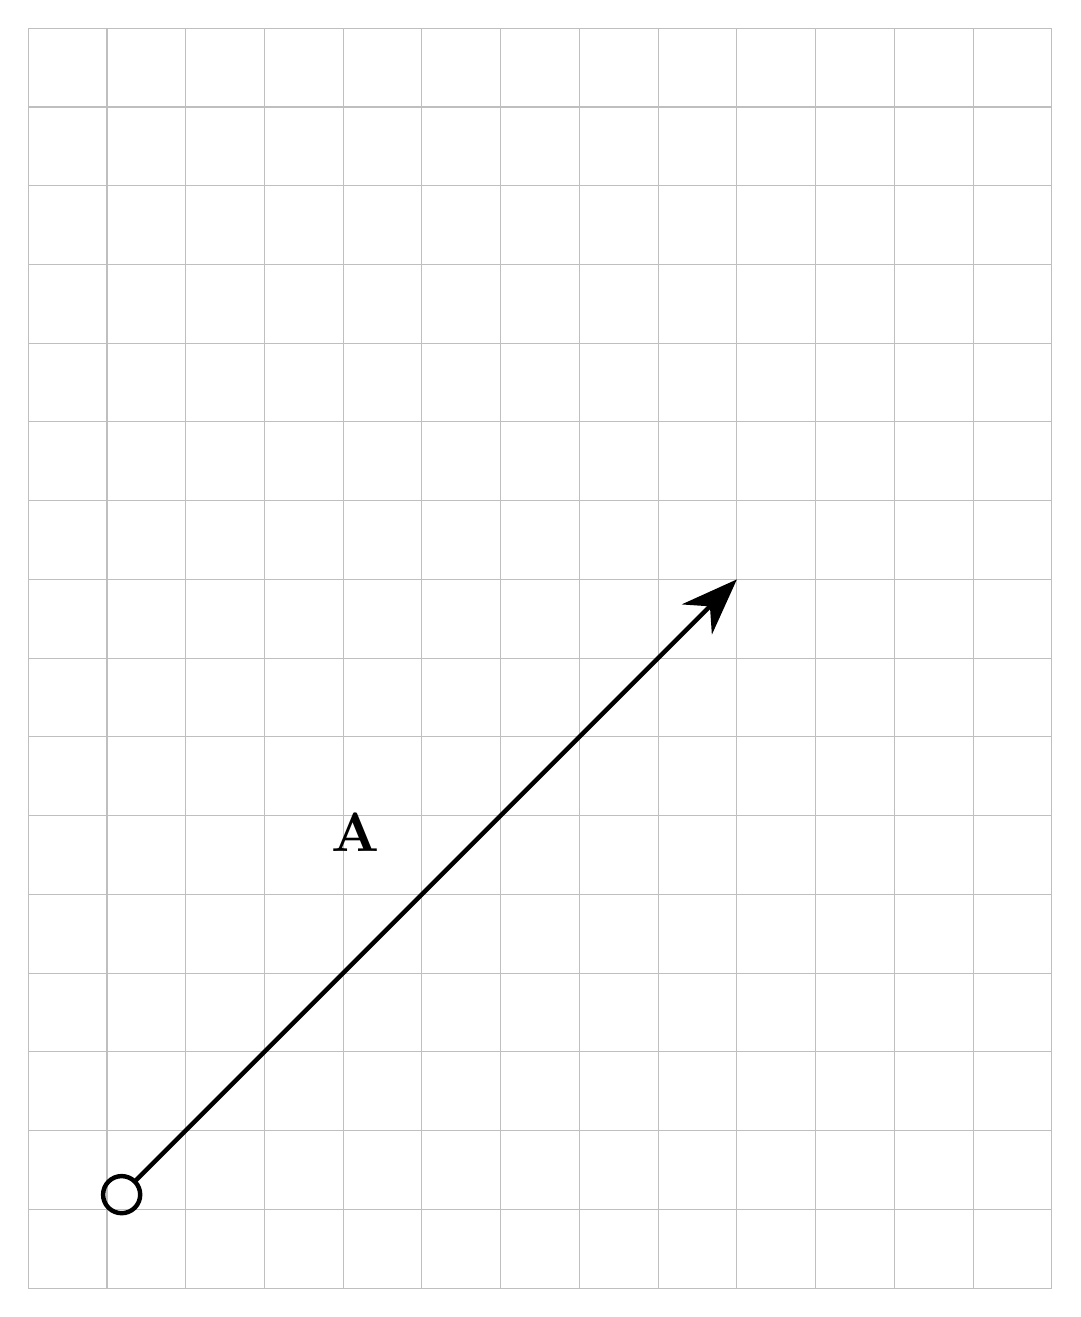
\begin{tikzpicture}
  \draw[step=1, lightgray] (0, 0) grid (13, 16);
  \draw[{Circle[scale=2, open]}-{Stealth[scale=2]}, 
  ultra thick] 
  (1, 1) -- (9, 9) 
  node[midway, above left=10pt, scale=2] {$\mathbf{A}$};
\end{tikzpicture}

\end{document}